%
% sesion6.tex
% 
% Copyright 2014 Rony J. Letona <zronyj@gmail.com>
% 
% This program is free software; you can redistribute it and/or modify
% it under the terms of the GNU General Public License as published by
% the Free Software Foundation; either version 2 of the License, or
% any later version.
% 
% This program is distributed in the hope that it will be useful,
% but WITHOUT ANY WARRANTY; without even the implied warranty of
% MERCHANTABILITY or FITNESS FOR A PARTICULAR PURPOSE.  See the
% GNU General Public License for more details.
% 
% You should have received a copy of the GNU General Public License
% along with this program; if not, write to the Free Software
% Foundation, Inc., 51 Franklin Street, Fifth Floor, Boston,
% MA 02110-1301, USA.
%

\documentclass[10pt,letterpaper]{article}
\usepackage[latin1]{inputenc}
\usepackage[spanish]{babel}
\usepackage{graphicx}
\usepackage{hyperref}
\usepackage{amsmath}
\usepackage{amsfonts}
\usepackage{amssymb}
\usepackage{color}
\usepackage{float}
\usepackage{upquote}
\usepackage[left=2cm,right=2cm,top=2cm,bottom=2cm]{geometry}
\author{Rony J. Letona}
\title{Taller de Computaci\'on Cient\'ifica para Ciencias Qu\'imicas: Sesi\'on 6}
\definecolor{light-gray}{gray}{0.90}

\newcommand{\tab}[1]{\hspace{.2\textwidth}\rlap{#1}}

\newcommand{\inlinecode}[1]{
\colorbox{light-gray}{\texttt{#1}}
}

\newsavebox{\selvestebox}
\newenvironment{Code}
{
\begin{lrbox}{\selvestebox}%
\begin{minipage}{\dimexpr\columnwidth-2\fboxsep\relax}
\fontfamily{\ttdefault}\selectfont
}
{\end{minipage}\end{lrbox}%
\begin{center}
\colorbox{light-gray}{\usebox{\selvestebox}}
\end{center}
}

\newcommand{\Picture}[3]
{
	\begin{figure}[H]
	\begin{center}
	\caption{#3}
	\includegraphics[scale=#2]{#1}
	\end{center}
	\end{figure}
}

\begin{document}
\maketitle

\section{Objetos, Paquetes y Algoritmos}
Al terminar un curso de programaci\'on que no nos gust\'o, generalmente nos sentimos aliviados y decidimos jam\'as volver a ver c\'odigo en nuestras vidas. Es m\'as, compadecemos al pobre amigo nuestro que decide meterse a estudiar cursos avanzados o la carrera de ingenier\'ia en sistemas. Pero muchas veces el problema m\'as grande no es que nos hayan dado mal el curso, sino que jam\'as nos mostraron que los principios de este se pod\'ian aplicar a algo en nuestra vida diaria. Por eso, esta vez, vamos a intentar darle prop\'osito a todo lo que hemos aprendido. Esta vez ya no vamos a enfocarnos en usar bien las cosas y vamos a asumir que podemos hacer lo que nos propongamos o vamos a aprender por nuestra cuenta lo necesario para lograrlo. Estos documentos se convertir\'an entonces en una gu\'ia de lo que podemos hacer despu\'es. Ya no vamos a entrar tanto en detalle del \emph{c\'omo} estamos haciendo algo. Ahora vamos a hacerlo para contestar el \emph{por qu\'e}. Nos vamos a enfocar entonces en ver qu\'e podemos crear con eso que hemos aprendido. Para ello vamos a comenzar por ver qu\'e significa eso de \emph{Programaci\'on Orientada a Objetos} y c\'omo es que, aunque no nos hayamos dado cuenta, ya la estamos usando. Luego seguiremos buscando realizar tareas de matem\'atica mediante algunos paquetes. Finalmente vamos a aprender sobre algoritmos y por qu\'e es una buena idea utilizarlos para tareas desde ordenar listas, hasta hallar la conformaci\'on m\'as estable de una mol\'ecula. Comencemos completando algo de la sesi\'on pasada.

\subsection{Ordenando Ideas: Programaci\'on Orientada a Objetos}
Hay una rama de programaci\'on que nos permite hacer mucho m\'as de lo que ya sabemos. Esta se llama \emph{Programaci\'on Orientada a Objetos}. La \emph{orientaci\'on a objetos} ha revolucionado la programaci\'on de maneras muy interesantes. Desde las interfaces gr\'aficas, hasta cambios de nombres cuando un lenguaje cambia por orientarse a objetos: de C a C++, de Pascal a Delphi, etc. La orientaci\'on a objetos nos permite hacer muchas cosas, y sin embargo, no es tan complicada. Una duda que surge muy seguido cuando comenzamos a programar es: Existe otro tipo de datos? O mejor a\'un: Puedo crear yo algo similar a mi propio tipo de dato como \inlinecode{int}, \inlinecode{boolean}, \inlinecode{string} o \inlinecode{float}? Eso ser\'ia muy interesante, puesto que podr\'ia crear cosas nuevas. Pero antes de empezar pregunt\'emonos por un momento, qu\'e es un objeto?\\

Un objeto es, para fines pr\'acticos, \textbf{algo}. Puede ser lo que nosotros querramos o necesitemos. Claro, cada objeto pertenece a una clase de objetos. Un l\'apiz es un objeto y pertenece a la clase de \emph{cosas para escribir}. Una manzana es un objeto que pertenece a una clase \emph{frutas}. Claro, cada objeto se diferencia por sus caracter\'isticas o lo que el objeto puede hacer. Un l\'apiz puede escribir, por ejemplo. Una manzana es roja, dulce y jugosa. Podemos hacer esto con cualquier objeto conocido! Pero, y esto qu\'e tiene que ver con programaci\'on? Es sencillo: la orientaci\'on a objetos nos permite hacer exactamente eso: crear clases de las que salgan objetos con propiedades especiales. Eso nos permite ordenar nuestras ideas.\\

Esta vez en el Taller, vamos a trabajar con qu\'imica, as\'i que vamos a intentar describir a los \'atomos y mol\'eculas como objetos. Veamos c\'omo hacer esto.

\subsubsection{Clases}
Comencemos entonces con lo m\'as grande. Necesitamos una clase de objetos: \inlinecode{Atomo} Para ello vamos a escribir lo siguiente en Python:

\begin{Code}
class Atomo:\\
\hspace*{4mm} pass
\end{Code}

En este momento, \inlinecode{pass} lo estamos usando solo para que la clase exista. Esta palabra no hace nada m\'as que existir. Sin embargo, ahora que hemos creado la clase, somos capaces de escribir \inlinecode{x = Atomo()} y veremos que efectivamente \inlinecode{x} se convierte en un objeto \inlinecode{Atomo}. Esto lo podemos comprobar al imprimir \inlinecode{x} Un dato curioso, sin embargo, es si le solicitamos a Python el tipo de dato de \inlinecode{x} Si hacemos esto, veremos que \inlinecode{x} es una instancia. Esto significa que \inlinecode{x} es una forma de \inlinecode{Atomo}, es decir, un objeto.\\

Veamos qu\'e m\'as se puede hacer con nuestro \'atomo. Por ahora vamos a darle propiedades. Vamos a decirle que su s\'imbolo es \textbf{H}, que su peso at\'omico es de $1.0079 g\ mol^{-1}$ y que tiene n\'umero at\'omico $1$. D\'emosle esas propiedades.

\begin{Code}
x.simbolo = "H"\\
x.peso = 1.0079\\
x.numeroato = 1
\end{Code}

Perfecto! Ahora si deseamos ver qu\'e contiene nuestro objeto, solo escribimos \inlinecode{dir(x)} y veremos lo que ya ingresamos. Tambi\'en vamos a hallar algunas otras cosas, pero no debemos de prestarles atenci\'on ahorita.\\

Crear objetos de esta manera es sencillo, pero no muy pr\'actico. Ser\'ia muy conveniente que pudieramos darle todas esas propiedades a nuestro objeto \inlinecode{Atomo} desde el principio. Pues para eso vamos a modificar un poco nuestra clase. Ahora vamos a escribirla de la siguiente manera:

\begin{Code}
class Atomo:\\
\hspace*{4mm} def \_\_init\_\_(self, simbolo = "H", peso = 1.0079, numero = 1):\\
\hspace*{10mm} self.simbolo = simbolo\\
\hspace*{10mm} self.peso = peso\\
\hspace*{10mm} self.numeroato = numero
\end{Code}

Qu\'e hicimos all\'i? Bueno, comenzamos creando la clase. Luego definimos una funci\'on \emph{dentro} de la clase. A continuaci\'on asignamos los argumentos de la funci\'on a valores \inlinecode{self}. Qu\'e es lo que pasa? Cuando definimos una funci\'on dentro de una clase, esta se pasa a llamar un m\'etodo. Ya veremos m\'as adelante qu\'e se puede hacer con ellos. Pero por ahora, nos interesa el m\'etodo \inlinecode{\_\_init\_\_} Este m\'etodo es el inicial. Es con el que una clase va a arrancar cuando sea instanciada (e.g. cuando escribimos \inlinecode{x = Atomo()}). Por otro lado, la palabra \inlinecode{self} se refiere a la clase misma. Vamos a ver c\'omo funciona y luego vamos a explicar paso a paso qu\'e es lo que hicimos. Ahora vamos a instanciar la clase de la siguiente forma:

\begin{Code}
y = Atomo("He", 4.002602, 2)
\end{Code}

Lo que est\'a sucediendo aqu\'i es que cuando instanciamos la clase esta vez, los valores que ingresamos dentro de \inlinecode{Atomo} est\'an entrando realmente en \inlinecode{\_\_init\_\_}. El m\'etodo est\'a pas\'andole estos valores a \inlinecode{self}, lo cual se refiere realmente a la clase. Lo que acabamos de hacer es entonces lo mismo que hab\'iamos hecho antes con el hidr\'geno, pero en vez de asignarle los valores uno por uno despu\'es de haber creado el objeto, lo hicimos de una vez. Podemos comprobar esto escribiendo \inlinecode{dir(y)}.\\

Si deseamos sacar alguno de los valores de \inlinecode{y}, solo debemos de escribir algo como \inlinecode{y.simbolo} o \inlinecode{y.peso} Veremos que el objeto tiene sus proiedades guardadas como variables. Un ejemplo sencillo a hacer ser\'ia intentar crear una clase \textbf{Fruta} de la cual instanciemos manzanas, peras, bananos, etc. con diferentes propiedades como color, tama\~no, sabor, etc.\\

Ya vimos c\'omo guardar propiedades dentro de un objeto partiendo de la clase y partiendo del objeto directamente. Ahora vamos a profundizar un poco en los m\'etodos.

\subsubsection{M\'etodos}
Los m\'etodos dentro de una clase en Python son simplemente funciones. Lo que sucede es que estas van a interactuar con las variables \emph{dentro} de la clase. Adem\'as, hay algunos m\'etodos que s\'i son especiales. Uno que ya vimos fue \inlinecode{\_\_init\_\_}. Pero no nos vamos a quedar all\'i. Podemos crear un m\'etodo \inlinecode{\_\_repr\_\_} que devuelva un \inlinecode{string}, por ejemplo. De ser as\'i, al momento de imprimir nuestro objeto, aparecer\'a lo que devuelva \inlinecode{\_\_repr\_\_}. As\'i hay muchos m\'etodos especiales que le confieren propiedades especiales a nuestros objetos. Entre ellos hay m\'etodos para sumar, restar, multiplicar, dividir, comparar, eliminar, etc. La idea es que podamos crear cosas nuevas. Un ejemplo claro son las matrices $\mathbb{R}^{n \times m}$. Veamos c\'omo podr\'iamos hacer algo as\'i, pero esta vez no copiemos ni intentemos esto en nuestro ordenador. Busquemos entender la forma y el concepto detr\'as de esto. En otras palabras, pong\'amosle atenci\'on solo a los comentarios, los nombres de la clase y de las funciones y los valores que retorna cada m\'etodo.\\

\begin{scriptsize}
\begin{Code}
class Matrix(list):\\
\hspace*{5mm} \# Metodo para representar la matriz\\
\hspace*{5mm} def \_\_repr\_\_(self):\\
\hspace*{11mm} c = len(self)\\
\hspace*{11mm} f = len(self[0])\\
\hspace*{11mm} out = " \textbackslash t"\\
\hspace*{11mm} for y in xrange(f):\\
\hspace*{17mm} for x in xrange(c):\\
\hspace*{23mm} out += str(round(self[x][y], 5)) + " \textbackslash t"\\
\hspace*{17mm} out += " \textbackslash n\textbackslash t"\\
\hspace*{11mm} return out\\
\\
\hspace*{5mm} \# Metodo para sumar\\
\hspace*{5mm} def \_\_add\_\_(self, other):\\
\hspace*{11mm} if self.check("\ \hspace*{-3mm} add", other):\\
\hspace*{17mm} new = [map(lambda r, s: r + s, i, j) for i, j in zip(self, other)]\\
\hspace*{17mm} return Matrix(new)\\
\hspace*{11mm} else:\\
\hspace*{17mm} raise TypeError, "Matrix: Dimensions do not match."\\
\\
\hspace*{5mm} \# Metodo para restar\\
\hspace*{5mm} def \_\_sub\_\_(self, other):\\
\hspace*{11mm} if self.check("\ \hspace*{-3mm} add", other):\\
\hspace*{17mm} new = [map(lambda r, s: r - s, i, j) for i, j in zip(self, other)]\\
\hspace*{17mm} return Matrix(new)\\
\hspace*{11mm} else:\\
\hspace*{17mm} raise TypeError, "Matrix: Dimensions do not match."\\
\\
\hspace*{5mm} \# Metodo para multiplicar\\
\hspace*{5mm} def \_\_mul\_\_(self, other):\\
\hspace*{11mm} if type(other) == int or type(other) == float:\\
\hspace*{17mm} new = [map(lambda r: other * r, i) for i in self]\\
\hspace*{17mm} return Matrix(new)\\
\hspace*{11mm} else:\\
\hspace*{17mm} if self.check("mul", other):\\
\hspace*{23mm} tra = self.transpose()\\
\hspace*{23mm} fa = len(tra)\\
\hspace*{23mm} cb = len(other)\\
\hspace*{23mm} new = [[0] * fa for t in xrange(cb)]\\
\hspace*{23mm} for f in xrange(fa):\\
\hspace*{29mm} for c in xrange(cb):\\
\hspace*{35mm} new[c][f] = sum(map(lambda r, s: r * s, tra[f], other[c]))\\
\hspace*{23mm} return Matrix(new)\\
\hspace*{17mm} else:\\
\hspace*{23mm} raise IndexError, "Matrix: Dimensions are not a match to multiply."\\
\\
\hspace*{5mm} \# Metodo para conocer las dimensiones de la matriz\\
\hspace*{5mm} def dim(self):\\
\hspace*{11mm} return len(self[0]), len(self)\\
\\
\hspace*{5mm} \# Metodo para revisar si las matrices cumplen con ciertas propiedades para poder ser operadas\\
\hspace*{5mm} def check(self, op, other):\\
\hspace*{11mm} if op == "\ \hspace*{-3mm} add"\ or op == "sub":\\
\hspace*{17mm} ia, ja = self.dim()\\
\hspace*{17mm} ib, jb = other.dim()\\
\hspace*{17mm} if ia == ib and ja == jb:\\
\hspace*{23mm} return True\\
\hspace*{17mm} else:\\
\hspace*{23mm} return False\\
\hspace*{11mm} elif op == "mul":\\
\hspace*{17mm} fila = len(self)\\
\hspace*{17mm} columna = len(other[0])\\
\hspace*{17mm} if fila == columna:\\
\hspace*{23mm} return True\\
\hspace*{17mm} else:\\
\hspace*{23mm} return False\\
\hspace*{11mm} else:\\
\hspace*{17mm} raise ValueError, "Matrix: There is no such operation."
\end{Code}
\end{scriptsize}

Aqu\'i definimos una clase matriz con un m\'etodo para cada operaci\'on b\'asica. Le definimos operaciones suma entre matrices, resta entre matrices y multiplicaci\'on tanto por una constante como por una matriz. Adem\'as de esto, le creamos un m\'etodo para poder representar las matrices como un arreglo. Casi todo el software de inform\'atica qu\'imica que calcula las coordenadas 3D de las mol\'eculas tiene que tener una clase siguiendo esta idea. Todos los m\'etodos que vimos ahorita nos permiten calcular operaciones como $M_a + M_b$ o $M_c \times M_d$ sin necesidad de llamar al m\'etodo directamente. Sin embargo, si quisieramos calcular la transpuesta de una matriz\footnote{Esto se refiere a invertir los valores de la matriz usando como eje la diagonal de la esquina superior izquierda hasta la esquna inferior derecha.}, tendr\'iamos que incluir un m\'etodo \inlinecode{transpose()} que nos permita hacer eso.

\begin{footnotesize}
\begin{Code}
\# Transposicion de una matriz\\
def transpose(self):\\
\hspace*{5mm} temp = zip(*list(self))\\
\hspace*{5mm} new = [list(e) for e in temp]\\
\hspace*{5mm} return Matrix(new)
\end{Code}
\end{footnotesize}

Entonces ya podr\'iamos calcular la transpuesta de una matriz $M^T$. Esto lo tendr\'iamos que hacer, sin embargo, de la siguiente manera: \inlinecode{M.transpose()}. As\'i podemos seguir creando m\'etodos dentro de nuestra clase o podemos guardar variables dentro de ella sin ning\'un problema. Una clase es entonces como cuando guard\'abamos datos y funciones en un archivo de Python y luego lo import\'abamos como librer\'ia. La diferencia es que la clase tiene algunas caracter\'isticas especiales como los m\'etodos de inicializaci\'on, representaci\'on u operaciones matem\'aticas.\\

Si deseamos probar lo que vimos aqu\'i (esto es opcional), copiemos la clase completa en un documento \emph{matriz.py}. Luego vamos a llamar a Python y vamos a importar Matrix de la siguiente manera \inlinecode{from matriz import Matrix} Unas cuantas operaciones que podr\'iamos probar son las siguientes:

\begin{Code}
m = Matrix([[ 1, 3,-5], [-1, 0,-3], [ 4, 1, 2]])\\
n = Matrix([[-7, 4, 9], [ 6,-1, 0], [-2,-3, 5]])\\
print( type( m ) )\\
print( m )\\
print( n )\\
print( m + n ) \# Suma de matrices\\
print( m * n ) \# Multiplicacion de matrices\\
print( m * 3 ) \# Multiplicacion por una constante\\
print( n.transpose() ) \# Transpuesta de la matriz
\end{Code}

\noindent Cu\'ales fueron los resultados? Notas algo que llama tu atenci\'on? Comenta con tu compa\~nero de al lado.\\

Podr\'iamos seguir probando todo lo que se puede hacer con esto, pero vamos a detenernos all\'i un momento. Con esto ya entendimos qu\'e es lo que hace la clase \inlinecode{Matrix}. Los m\'etodos nos son invisibles, y sin embargo, funcionan. Podemos hacer operaciones matem\'aticas con facilidad y nos podemos dar cuenta que nuestro ordenador es capaz de hacer esto en tiempos relativamente cortos. Qu\'e otro uso le podr\'ias dar a las clases y los objetos? Te interesar\'ia construir uno, o preferir\'ias seguir trabajando con funciones y documentos separados? Hallas alguna ventaja? Comenta un momento con tu compa\~nero de al lado.

\subsection{Haciendo un poco de Matem\'atica}
El \'ultimo d\'ia que nos vimos terminamos mostrando una serie de paquetes que podemos usar para hacer una serie de operaciones matem\'aticas de diferente tipo. Hoy vamos a entender un poco mejor sobre c\'omo podemos hacer un mejor uso de ellos y por qu\'e es conveniente usarlos a veces. Por ahora nos vamos a enfocar en resolver algunos problemas de matem\'atica que suelen molestarnos a veces cuando estamos llevando alg\'un curso.\\

Para esta parte del taller, vamos a cambiar a un ambiente un poco m\'as especializado. Vamos a comenzar a trabajar en cuadernos de notas que nos pueden servir posteriormente como referencias personales. En otras palabras, ser\'a una buena idea de que detallemos bien nuestros cuadernos de notas e incluyamos desde conceptos hasta dudas, para poderlos usar mejor en el futuro. Para ello vamos a abrir una l\'inea de comando nueva, y vamos a escribir \inlinecode{ipython notebook} Luego vamos a esperar un momento. Nuestro navegador se va a abrir y vamos a ver una nueva interfaz.\\

Lo que haremos ahora es sencillo: vamos a crear un nuevo cuaderno. Hacemos click en donde dice \textit{New Notebook} y vamos a ver nuestro nuevo cuaderno de notas. Esta alternativa suele ser m\'as c\'omoda para trabajar proyectos, porque en \'el se puede ir creando desde c\'odigo \emph{dentro} de un documento con texto, hasta incluir gr\'aficas, animaciones, etc. Los cuadernos de IPython\footnote{El proyecto IPython evolucion\'o para poder utilizar m\'as lenguajes de programaci\'on: Julia, Python, R. Por esta raz\'on el proyecto ahora se llama Jupyter. Si en alg\'un momento nos topamos con \'el, recordemos que la plataforma Jupyter es b\'asicamente igual a IPython.} ser\'an ahora nuestro lugar ideal de trabajo. Comencemos a trabajar.\\

Lo primero que vamos a escribir en la celda es \emph{Ejercicios de Matematica con IPython}. Luego iremos a donde dice \textit{Code}, abriremos el men\'u y vamos a seleccionar \textit{Heading 1}. Finalmente vamos a hacer click en la flecha hacia la derecha (como si estuvi\'eramos reproduciendo la celda). Inmediatamente veremos que lo que escribimos se acaba de transformar en algo m\'as presentable. Lo mismo podemos hacer con las dem\'as opciones: \textit{Heading 2}, \textit{Heading 3}, \textit{Raw text}, \textit{Markdown}, etc. Habr\'ia que aclarar que \textit{Raw text} dejar\'a el texto as\'i como lo escribimos, sin ponerlo m\'as presentable. \textit{Markdown}, por otra parte, tiene una sintaxis un poco diferente. Este nos permite formatear el texto de maneras muy diversas, pero debemos de saber c\'omo es que se hace esto\footnote{Para eso podemos abrir el documento \textit{Markdown.ipynb} en la carpeta \textit{Data} del taller.}.\\

Ahora, vamos a dedicar una celda solo para poder importar lo necesario para trabajar esta vez. En nuestra nueva celda, vamos a escribir:

\begin{Code}
\%pylab inline\\
from sympy import *\\
init\_printing()\\
import numpy
\end{Code}

Algunas de las cosas que ponemos ac\'a ya las hemos visto. Otras no. No nos enfoquemos tanto en esto ahora, sino en lo que nos va a permitir hacer esto. Si deseamos profundizar sobre la sintaxis de IPython y el por qu\'e de cada comando que acabamos de escribir, podemos estudiarlo en los tutoriales que se nos ofrecen en su p\'agina \href{http://ipython.org/}{IPython}. Otra alternativa, y es en lo que el taller de hoy se basa, son los cursos ofrecidos como cuadernos de notas: \href{https://github.com/jrjohansson/scientific-python-lectures}{Python Scientific Lectures}. Pero por ahora, lo que nos interesa m\'as es poder seguir trabajando para poder llegar a hacer qu\'imica con estas herramientas.\\

Lo primero que haremos ser\'a intentar realizar aquellos ejercicios de los cursos b\'asicos de matem\'atica que llevamos en nuestros \'ultimos a\~nos de colegio y primeros a\~nos universitarios. Vamos a comenzar definiendo una variable nueva para poder hacer algo de \'algebra: \inlinecode{x = Symbol("x")} Luego, en la l\'inea de abajo, vamos a escribir una de esas funciones que nos pon\'ian a analizar: \inlinecode{f = x**2 - 6*x + 2}. Finalmente solo escribiremos \inlinecode{f} en la \'ultima l\'inea y presionaremos \textbf{Shift + Enter}. Lo primero que vamos a ver es la funci\'on que acabamos de definir, pero utilizando una tipograf\'ia\footnote{Tipograf\'ia es el tipo de letra. Como los que podemos escoger en Microsoft Word al escribir un documento (e.g. Arial, Times New Roman).}\\

Para continuar, lo que vamos a hacer es simple. Vamos a graficar la funci\'on, hallar en d\'onde cruza esta el eje x (i.e. hallaremos sus ceros) y a hallar su valor m\'as peque\~no (i.e. el valor m\'inimo). Este ejercicio ya nos tomar\'ia unos 5 minutos si somos r\'apidos. La idea es que con lo que vamos a hacer ahorita, vamos a invertir los mismos 5 minutos una \'ultima vez. Luego veremos la ventaja de crear un peque\~no programa para hacerlo por nosotros.\\

\noindent Vamos por pasos entonces. Primero vamos a graficar la funci\'on. Para eso necesitamos que nuestro ordenador interprete todo como n\'umeros. Generalmente para graficar, hac\'iamos una tablita e \'ibamos escogiendo puntos en x y luego calculando los puntos en y. Intentaremos hacer lo mismo ahora, pero autom\'aticamente.

\begin{footnotesize}
\begin{Code}
x\_vec = arange(-2, 10, 0.5) \# Aqui creamos una lista especial desde -2 hasta 10 en intervalos de 0.5 para el eje x\\
y\_vec = numpy.array([N(f.subs(x, xx)) for xx in x\_vec]) \# Y aqui creamos una nueva lista tipo numpy con los valores en y
\end{Code}
\end{footnotesize}

\noindent Para ver nuestra tablita, solo es necesario escribir \inlinecode{x\_vec} o \inlinecode{y\_vec} en una celda y presionar Shift + Enter. La primera nos mostrar\'a los valores en x y la segunda los valores en y. Lo importante del c\'odigo que acabamos de escribir son los n\'umeros que escogimos como puntos en x: -2, 10 y 0.5. Qu\'e pasar\'a si cambiamos alguno? Probemos y veamos el resultado. Lo dem\'as podemos dejarlo a un lado por ahora. Continuando, vamos a crear la gr\'afica.

\begin{footnotesize}
\begin{Code}
fig, ax = subplots() \# Creamos un cuadro vacio en el cual vamos a colocar nuestra grafica\\
ax.set\_title("Primera grafica") \# Le ponemos nombre a nuestra grafica (pongamosle otro nombre si asi queremos)\\
ax.set\_xlabel("x") \# Colocamos el nombre del eje x (podemos ponerle como querramos)\\
ax.set\_ylabel("f(x)") \# Colocamos el nombre del eje y (tambien podemos ponerle como querramos)\\
ax.plot(x\_vec,y\_vec,"b-") \# Y graficamos la funcion basandonos en los puntos\\
ax.grid(True, which='both') \# Agregamos una cuadricula para entender mejor por donde pasa la grafica
\end{Code}
\end{footnotesize}

\noindent Ejecutemos esto con Shift + Enter y veamos qu\'e es lo que pasa.

\begin{figure}[H]
\begin{center}
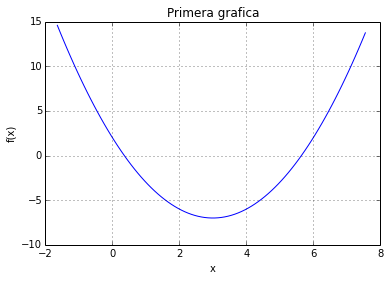
\includegraphics[scale=0.5]{img/graf1.png}
\end{center}
\end{figure}

\vspace*{-6mm}

\noindent Es importante notar que al graficar (el \'ultimo paso), incluimos una \emph{b} y un gui\'on en lo que escribimos. Probemos cambiar la \emph{b} por una \emph{r}, una \emph{g} o una \emph{k}. O mejor a\'un, probemos cambiar el gui\'on por dos, o por un asterisco y un gui\'on. Tambi\'en se puede con una \textbf{v}, una \textbf{o} o una \textbf{x}. Intentemos alguno de esos cambios y veamos qu\'e sucede. Luego comentemos con nuestros dem\'as compa\~neros.\\

\noindent Una vez con la gr\'afica ya frente a nosotros, podemos continuar hallando todo lo dem\'as. Primero, los ceros. Para ello vamos a pedirle a nuestro ordenador que resuelva la funci\'on como si fuera una ecuaci\'on igualada a 0.

\begin{footnotesize}
\begin{Code}
z = solve(f, x) \# Notemos que no es necesario igualar a 0 explicitamente. Nuestro ordenador siempre iguala a 0 la expresion que pongamos.\\
z
\end{Code}
\end{footnotesize}

\noindent Para mostrar el resultado es que agregamos la \emph{z} al final. Nuestro ordenador no nos devuelve n\'umeros nada m\'as. Nos devuelve las expresiones algebr\'aicas en las ra\'ices sin desarrollar. Adem\'as, \emph{z} es ahora una lista con nuestros valores. Los vamos a usar despu\'es. Pero por ahora, hallemos la derivada y el m\'inimo de nuestra funci\'on.

\begin{footnotesize}
\begin{Code}
derivada = f.diff(x) \# Aqu\'i derivamos nuestra funci\'on con respecto de x\\
derivada
\end{Code}
\end{footnotesize}

\noindent Ya con la derivada, ahora solo es de igualar el resultado a 0 y resolver para hallar el m\'inimo. Pero eso ya vimos c\'omo hacerlo:

\begin{footnotesize}
\begin{Code}
solve(derivada, x) \# Resolvemos nuestra derivada igualada a 0 con respecto a x
\end{Code}
\end{footnotesize}

\noindent Excelente! Si ahora ya sabemos d\'onde est\'a el punto m\'as bajo de nuestra funci\'on. Por ahora, sacar derivadas y resolver ecuaciones no creo que haya sido m\'as f\'acil excepto, quiz\'a, con alguna calculadora. Sin embargo, no nos quedaremos all\'i. Para terminar vamos a hallar el \'area comprendida entre los el eje x y la funci\'on justo entre los dos valores que hallamos antes como ceros. En otras palabras, vamos a integrarla.

\begin{footnotesize}
\begin{Code}
area = f.integrate((x, z[0], z[1])) \# Le decimos a nuestro ordenador que queremos integrar nuestra funcion con respecto de x, desde un cero hasta el otro\\
area
\end{Code}
\end{footnotesize}

\noindent Claro, el resultado as\'i no nos va a gustar. Verlo como expresi\'on algebr\'aica no es lo que ten\'iamos en mente cuando busc\'abamos el \'area. Sin embargo, para obtener la cifra no es necesario calcularla a mano. Solo escribimos \inlinecode{N(area, 6)} para obtener el n\'umero real con 6 cifras significativas. El valor ser\'a negativo porque el \'area queda por debajo del eje x, pero la cifra ser\'a la correcta.\\

Llegamos al final de esta secci\'on y al momento m\'as importante. Qu\'e pasa si nos dicen ahora que queremos hallar todo lo anterior, pero de la funci\'on $f(x) = x^2 - x - 1$? Pues en vez de reescribir todo lo que ya hicimos, solo cambiamos la funci\'on al principio y reiniciamos nuestro cuaderno de notas. Quiz\'a cambiar de d\'onde a d\'onde queremos graficar ser\'ia conveniente. Pero en general, ya hicimos un peque\~no script que nos permite hallar muchas cosas que antes nos hubieran tomado mucho tiempo. Claro, este programa funciona solo para par\'abolas, pero es adaptable a cualquier funci\'on si as\'i lo deseamos.\\

Perfecto! Ahora nos hemos dado cuenta de que nuestro ordenador puede hacer muchas m\'as cosas que solo programaci\'on. Puede hacer matem\'atica. Si deseamos entrar m\'as en detalle de lo que se puede hacer en esto, es recomendable revisar las dos referencias que nos dieron al principio. Solo es conveniente mencionar que se puede simplificar expresiones algebr\'aicas, desarrollarlas, calcular sumatorias, productorias, series, series de potencias, l\'imites, fracciones parciales, estad\'istica, c\'alculo multivariable, \'algebra de vectores y matrices y mec\'anica cu\'antica. Tambi\'en podemos visualizar varios tipos de gr\'aficas, incluyendo de barras, de llenado, de dispersi\'on, curvas de nivel, gr\'aficas en coordenadas polares, mapas de densidad y hasta superficies en 3D. Y si eso se queda corto, IPython tambi\'en nos permite hacer animaciones sencillas para simular fen\'omenos.

\subsection{Algoritmos}
Para continuar vamos a entrar a un tema un poco m\'as bonito. A pesar de que para muchos escuchar el t\'ermino \emph{algoritmo} sea ya motivo de asustarse, no nos preocupemos. Nosotros ya vivimos utilizando algoritmos todos los d\'ias de nuestras vidas. Desde c\'omo hacer divisiones, hasta c\'omo hacer un pastel. Desde c\'omo hacer una titulaci\'on, hasta c\'omo desbloquear nuestro tel\'efono y poner m\'usica en \'el. Un algoritmo no es m\'as que una sucesi\'on de instrucciones que, al seguirlas, nos llevar\'an a solucionar un problema o calcular alguna cantidad espec\'ifica.\\

En nuestro caso en particular, podr\'iamos decir que un algoritmo va a ser un peque\~no programa o una funci\'on a la que le daremos ciertos datos, ella calcular\'a algo con ellos siguiendo una secuencia de pasos, y se nos devolver\'an algunos resultados. En esta secci\'on vamos a ver c\'omo es que funcionan algunos algoritmos. No vamos a tratar de ide\'arnolas para crearlos, sino que simplemente buscaremos verlos y entenderlos. La idea ser\'a entonces entender para qu\'e sirven, qu\'e implica utilizarlos y por qu\'e es que tienen ciertas ventajas y desventajas. Vamos a proceder entonces del m\'as sencillo al m\'as complicado. Para ello vamos a seguir utilizando el mismo notebook de IPython.

\subsubsection{Hallando el M\'aximo en una Lista}
Este algoritmo es quiz\'a uno de los m\'as sencillos que hay. La idea es hallar el valor m\'as grande en una lista. Primero tomamos una lista con elementos num\'ericos. Luego, tomamos el primer valor como el m\'as grande. Ahora vamos a ir recorriendo la lista de manera c\'iclica, elemento por elemento, y revisando si el n\'umero que hallamos a continuaci\'on es m\'as grande al que ya llevamos como mayor. Si es m\'as grande, tomamos este como mayor. Si no, seguimos con el que ten\'iamos antes. Suena sencillo, no? Ve\'amoslo funcionar en c\'odigo.

\begin{small}
\begin{Code}
from numpy import random \# Importamos una libreria para generar numeros pseudo-aleatorios\\
l = random.randn(1, 50) \# Y luego generamos una lista de 50 numeros aleatorios\\
l \# Aqui los podemos ver
\end{Code}
\end{small}

Como nos podemos dar cuenta, el resultado es una lista dentro de otra lista. Esto hay que tomarlo muy en cuenta para poder continuar. Ahora vamos a ver el algoritmo en s\'i.

\begin{small}
\begin{Code}
maximo = l[0][0] \# Tomamos el primer elemento de la lista como maximo\\
for i in l[0]: \# Revisamos cada elemento de la lista de manera ciclica\\
\hspace*{4mm} if i >\ maximo: \# Si el elemento es mayor al maximo ...\\
\hspace*{12mm} maximo = i \# ... el nuevo maximo es ese elemento\\
maximo \# Miramos el resultado
\end{Code}
\end{small}

Ese es todo el algoritmo! Nada m\'as. Ahora, si nos ponemos a pensar detenidamente, lo \'unico que necesitar\'iamos ser\'ia colocar este peque\~no algoritmo dentro de una funci\'on y listo: tenemos la funci\'on \inlinecode{max()} que hab\'iamos visto la sesi\'on anterior. Pasemos ahora a otro algoritmo; uno un poco m\'as complicado.

\subsubsection{Ordenando una Lista de Datos}
El siguiente algoritmo que vamos a ver nos ayudar\'a a ordenar la lista que generamos hace un momento. Por eso mismo, partiremos del hecho de convertirlo en una funci\'on que le vamos a aplicar a nuestra lista. Aprovech\'andonos de que Python es muy flexible y que la eficiencia del uso de memoria y procesamiento no son algo importante a considerar ahorita, vamos a utilizar un algoritmo que no va a ordenar la lista exactamente, sino que va a crear una nueva lista con los elementos ordenados de la anterior. Para ello las instrucciones ser\'an as\'i:

\begin{enumerate}
\item Crear una lista nueva sin datos.
\item Buscar el m\'aximo en nuestra lista.
\item Agregar ese dato a la lista nueva.
\item Eliminar ese dato de nuestra lista.
\item Repetir 2, 3 y 4 hasta que no queden datos en nuestra lista.
\item Devolver lista nueva.
\end{enumerate}

No hay nada muy complicado dentro de lo que estamos haciendo aqu\'i. Lo \'unico que vale la pena mencionar es que necesitamos alguna manera de ir removiendo datos de una lista. Buscar el dato m\'as grande es algo que ya aprendimos hacer. La \'unica diferencia es que ahora necesitaremos que nuestro algoritmo pasado sea una funci\'on y que esta nos devuelva el \'indice del n\'umero m\'as grande, y no solo el valor del n\'umero. Veamos ahora el c\'odigo para entender un poco mejor.\\

\noindent La primera funci\'on, que ser\'ia lo mismo que hab\'iamos hecho para hallar m\'aximos, se va a ver as\'i:

\begin{footnotesize}
\begin{Code}
def maxim(lista):\\
\hspace*{5mm} maximo = lista[0]\\
\hspace*{5mm} ctrl = 0\\
\hspace*{5mm} for i in xrange(len(lista)):\\
\hspace*{11mm} if lista[i] > maximo:\\
\hspace*{17mm} maximo = lista[i]\\
\hspace*{17mm} ctrl = i\\
\hspace*{5mm} return maximo, ctrl
\end{Code}
\end{footnotesize}

\noindent Con ella podemos hallar no solo el m\'aximo, sino que tambi\'en hallamos en d\'onde se encuentra. Eso nos ser\'a \'util para saber qu\'e elemento de la lista original quitar. Ahora vamos a proceder con el algoritmo de ordenado.

\begin{footnotesize}
\begin{Code}
def ordenar(lista):\\
\hspace*{5mm} neo\_lista = []\\
\hspace*{5mm} while len(lista) >= 1: \# Si la lista es mayor o igual a uno ...\\
\hspace*{11mm} maximo, ctrl = maxim(lista) \# ... calcular el maximo ...\\
\hspace*{11mm} neo\_lista.append(maximo) \# ... insertarlo en la nueva lista ...\\
\hspace*{11mm} lista.pop(ctrl) \# ... y sacarlo de la lista original.\\
\hspace*{5mm} return neo\_lista
\end{Code}
\end{footnotesize}

\noindent Con esto ya podemos ordenar nuestra lista de datos anterior. Lo primero que habr\'ia que hacer es transformarla a una lista de Python normal: \inlinecode{datos = l.tolist()[0]}, y luego correr nuestro algoritmo llam\'andolo como funci\'on sobre nuestra nueva lista: \inlinecode{ordenar(datos)}. Este algoritmo es bastante sencillo de entender. Discutamos con nuestro compa\~nero de al lado a ver si nuestro c\'odigo se puede excribir m\'as eficientemente y qu\'e m\'as podr\'ia hacer con \'el.\\

Este es un buen momento para analizar la manera en que estamos ordenando. Estamos creando una lista nueva y estamos agreg\'andole elementos. Estas tareas son algo complicadas para nuestro ordenador si analizamos el proceso detenidamente. Al crear una lista nueva, estamos ocupando nuevo espacio en memoria, lo cu\'al requiere de m\'as tiempo. Cada vez que hacemos que una lista crezca y otra decrezca, el tiempo tambi\'en va a aumentar, ya que cada cambio requiere m\'as cambios en memoria. Este es, de hecho, el gran problema de las bases de datos. Por eso existen otros algoritmos m\'as eficientes. Algunos ejemplos de ellos son los algoritmos QuickSort, HeapSort y MergeSort.\\

En el caso del primero, el algoritmo implica escoger un dato al azar dentro de la lista e intercambiar los elementos a modo que los mayores a \'el queden del lado derecho y los menores del lado izquierdo. Terminado esto, repite el mismo proceso en cada lado de la lista nuevamente. Luego otra vez, y otra vez y as\'i sucesivamente hasta que solo queda ordenando pares de datos. La idea del QuickSort, si nos damos cuenta, es ir dividiendo el problema en pedazos e ir trabajando cada pedazo por separado acelerando el proceso y sin necesidad de crear o eliminar listas; solo se estuvo intercambiando datos de posici\'on. Este tipo de algoritmos son un tema de inter\'es actual en inform\'atica y en el manejo de bases de datos muy grandes.

\subsubsection{Bisecci\'on}
Un problema que generalmente no nos imaginamos sea complicado de resolver cuando lo hacemos con una calculadora es calcular una raiz cuadrada. En esta parte vamos a intentar calcular la raiz cuadrada de 3 haciendo uso de un algoritmo. El concepto de este es sumamente simple, pero primero tenemos que hacer un cambio sencillo en nuestra forma de pensar el problema. La idea ser\'a buscar el n\'umero $x$ que haga la siguiente expresi\'on verdadera: $x^2 - 3 = 0$. Si nos damos cuenta, al resolver la ecuaci\'on, estamos hallando la raiz de 3. Pero por ahora, nos servir\'a ver el problema de esta manera. De hecho, lo que vamos a hacer es plantear una funci\'on: $f \left( x \right) = x^2 - 3$ e ir buscando el valor de $x$ que nos lleve a que la funci\'on sea $0$. La idea es simple. Vamos a escoger dos valores $a$ y $b$ entre los que esperamos hallar el valor de $x$ y comenzaremos con el algoritmo.

\begin{enumerate}
\item Calcular $f \left( a \right)$ y $f \left( b \right)$.
\item Si hay diferencia de signo (uno es positivo y el otro negativo) entre los dos valores, seguimos. Si no, alegamos que hay error.
\item Calcular un nuevo valor $c$ que se halle en medio de $a$ y $b$ y calcular $f \left( c \right)$.
\item Si $f \left( c \right)$ tiene el mismo signo que $f \left( a \right)$, entonces $a$ toma ahora el valor de $c$.
\item Si $f \left( c \right)$ tiene el mismo signo que $f \left( b \right)$, entonces $b$ toma ahora el valor de $c$.
\item Si $f \left( c \right)$ es igual a $0$, devolver $c$.
\item Repetir los pasos del 3 al 6, hasta que $\left| b - a \right|$ sea menor a un n\'umero $e$ que nosotros establezcamos.
\end{enumerate}

En resumen, lo que estamos haciendo es ir partiendo a la mitad la distancia entre $a$ y $b$ dejando la raiz dentro de ese rango. Seguimos y seguimos hasta que estemos \textbf{muy} cerca del valor real. Veamos ahora el c\'odigo de esto.

\begin{footnotesize}
\begin{Code}
def biseccion(f, a, b, e):\\
\hspace*{5mm} a,  b = float(a), float(b)\\
\hspace*{5mm} if f(b)/f(a) >\ 0:\\
\hspace*{11mm} print "Los limites estan mal definidos"\\
\hspace*{11mm} return None\\
\hspace*{5mm} iteraciones = 0 \# Contador de iteraciones del algoritmo\\
\hspace*{5mm} while abs(b - a) >\ e: \# Revisar si ya pasamos de la cantidad de cifras significativas que deseamos\\
\hspace*{11mm} iteraciones += 1\\
\hspace*{11mm} c = (b - a)/ 2 + a\\
\hspace*{11mm} if f(c)/f(a) >\ 0:\\
\hspace*{17mm} a = c\\
\hspace*{11mm} elif f(c)/f(b) >\ 0:\\
\hspace*{17mm} b = c\\
\hspace*{11mm} elif f(c) == 0:\\
\hspace*{17mm} return c\\
\hspace*{5mm} print iteraciones\\
\hspace*{5mm} return c
\end{Code}
\end{footnotesize}

En este ya no se incluyen tantos comentarios para que nosotros comencemos a buscar entender cada parte. Hay, sin embargo, un par de cosas que vale la pena notar. Una de ellas es que vamos contando las iteraciones que hace el algoritmo. Otra es que la funci\'on que estamos ingresando, es de hecho, una \emph{funci\'on} de Python. Por ende, si deseamos probar nuestro nuevo algoritmo, debemos crear primero nuestra funci\'on de esta manera:

\begin{footnotesize}
\begin{Code}
def f(x):\\
\hspace*{5mm} return x**2 - 3
\end{Code}
\end{footnotesize}

Ahora, para probar nuestro algoritmo, solo escribimos: \inlinecode{biseccion(f, 1, 2, 1e-15)} Quiz\'a le tome un momentito a nuestro ordenador calcular esto, pero el resultado saldr\'a relativamente r\'apido. Qu\'e es lo que hicimos? Le dijimos que utilizara el algoritmo entre 1 y 2, y que parara cuando la diferencia entre $a$ y $b$ fuera menor a $1\cdot10^{-15}$. Considerando que nuestro ordenador calcula solo hasta 16 d\'igitos, 15 parece ser un buen n\'umero para detenerse. Si le pidi\'eramos 16, jam\'as parar\'ia porque no puede comparar un valor m\'as all\'a del d\'igito 16.\\

Al terminar el c\'alculo, vamos a notar que el algoritmo nos devuelve 2 n\'umeros: la cantidad de iteraciones y el resultado. Tomemos nota de la cantidad de iteraciones, porque nos servir\'an m\'as adelante. Ahora, para revisar si el resultado est\'a correcto, calculemos \inlinecode{3**0.5} en la siguiente celda y veamos qu\'e tan buen resultado nos qued\'o.

\subsubsection{M\'etodo de Newton}
El algoritmo anterior nos permiti\'o calcular la raiz de 3 en m\'as o menos 50 iteraciones. Ahora, a pesar de que nuestros procesadores son bastante r\'apidos y nosotros ni nos damos cuenta de cada vuelta del ciclo en nuestro programa, esto es poco eficiente. 50 vueltas para calcular un valor tan sencillo no parece ser muy rentable en costos de c\'omputo. La forma sencilla de pensar esto es: Har\'iamos nosotros 50 operaciones de esas a mano sin una calculadora? En el caso en que no querramos, aqu\'i vamos a proponer utilizar otro m\'etodo.\\

Hay una forma muy particular de hallar raices mediante una f\'ormula que vamos a ver a continuaci\'on. C\'omo llegar a esa f\'ormula es algo que podemos leer en cualquier libro de m\'etodos num\'ericos, as\'i que no lo cubriremos aqu\'i. Lo que dice esto es que podemos calcular el siguiente valor de $x$ a partir del anterior y haciendo uso de la funci\'on que ten\'iamos de la parte anterior y la derivada de la funci\'on. La f\'ormula se ve as\'i:

\begin{equation}
x_{n+1} = x_n - \frac{f \left( x_n \right)}{f' \left( x_n \right)}
\end{equation}

El problema es entonces la derivada. Pero como ya sabemos que si usamos SymPy nuestro problema se arregla, vamos a importar el paquete y vamos a comenzar trabajando con c\'alculo directamente: \inlinecode{from sympy import *} Ahora nos toca definir nuestra variable y nuestra funci\'on:

\begin{footnotesize}
\begin{Code}
x = Symbol("x")\\
f = x**2 - 3
\end{Code}
\end{footnotesize}

Ahora la idea ser\'a seguir los siguientes pasos para poder hallar la raiz:

\begin{enumerate}
\item Calcular la derivada de la funci\'on.
\item Calcular el nuevo valor de $x$ en base a un $x$ que ya tenemos (el primero lo tenemos que elegir nosotros) utilizando la f\'ormula que acabamos de ver.
\item Calcular la diferencia entre el $x$ anterior y el nuevo y comparar este contra otro valor que hayamos escogido.
\item Repetir pasos 2 y 3 hasta que la diferencia calculada en 3 sea m\'as peque\~na que el valor ingresado.
\item Devolver el valor de $x$.
\end{enumerate}

Ahora que ya tenemos una idea de c\'omo funciona este algoritmo, vamos a comenzar a revisar el c\'odigo. Vamos a notar que al igual que se reduce el n\'umero de pasos en el razonamiento, se reduce el tama\~no del c\'odigo.

\begin{footnotesize}
\begin{Code}
def NR(f, z, e=1e-9):\\
\hspace*{5mm} deriv = f.diff(x) \# Calculamos la derivada de la funcion\\
\hspace*{5mm} z0 = z \# Establecemos el valor inicial\\
\hspace*{5mm} z1 = z0 - N(f.subs(x, z0)/deriv.subs(x, z0)) \# Calculamos el primero valor despues del inicial\\
\hspace*{5mm} iteraciones = 1 \# Ya calculamos un valor, en tonces nuestro numero de vueltas es 1\\
\hspace*{5mm} while abs(z1 - z0) > e:\\
\hspace*{11mm} z0 = z1\\
\hspace*{11mm} z1 = N(z0 - f.subs(x, z0)/deriv.subs(x, z0))\\
\hspace*{11mm} iteraciones += 1\\
\hspace*{5mm} print iteraciones\\
\hspace*{5mm} return z1
\end{Code}
\end{footnotesize}

Eso es todo! No necesitamos m\'as. Hay algo interesante del momento en que declaramos la funci\'on: pusimos que uno de los valores es igual a \inlinecode{1e-9}, lo cual es igual a  $1 \cdot 10^{-9}$. Este ser\'a entonces el valor predeterminado de la funci\'on. Si no incluimos un tercer argumento, nuestro ordenador asume ese como el valor predeterminado para trabajar.\\

Ahora que ya entendimos mejor el c\'odigo, probemos correr nuestra funci\'on: \inlinecode{NR(f, 2, 1e-15)} Nos vamos a dar cuenta, casi de inmediato, que el algoritmo de Newton-Raphson es mucho m\'as eficiente que el de bisecci\'on. Este solo necesit\'o de 5 iteraciones para llegar al mismo resultado que el algoritmo anterior. En nuestro caso, la ventaja es que existen varios paquetes para hacer c\'alculo y eso nos evita calcular la derivada y evaluarla. En el caso de no contar con eso, tenemos que ingresar la derivada de \emph{cada} funci\'on al sistema para que nuestro ordenador sepa con qu\'e trabajar.

\subsubsection{M\'etodo de MonteCarlo}
Hasta ahorita hemos visto c\'omo trabajar con cosas sencillas: calcular una raiz, ordenar listas y hallar m\'aximos (o m\'inimos con un leve cambio de signo). Hallar una derivada o una integral suena a algo m\'as complicado, y sin embargo, no lo es. En este caso vamos a calcular una integral. De hecho, vamos a buscar el valor de $\pi$ a trav\'es de una integral. El resultado no ser\'a tan exacto, porque el m\'etodo no es el indicado para hallar muchos decimales, pero s\'i hallaremos una aproximaci\'on.\\

La idea es entonces plantear la ecuaci\'on de un c\'irculo: $f\! \left(x\right) = \sqrt{1 - x^2}$, la cual podemos definir en Python como \inlinecode{g = sqrt(1 - x**2)} Esta es la ecuaci\'on de un c\'irculo unitario (i.e. un c\'irculo de radio 1). Ahora, si recordamos bien, la f\'ormula para hallar el \'area de un c\'irculo es $A = \pi r^2$. Sin embargo, al intentar hallarla por integrales, tendr\'iamos que plantear la integral:

\begin{equation}
A = 2 \cdot \int_{-1}^{1} \sqrt{1 - x^2}  dx
\end{equation}

\noindent Claro, ser\'ia m\'as sencillo solo calcular un cuarto del c\'irculo y multiplicarlo por cuatro! Eso lo veremos m\'as adelante.\\

La idea es hallar el \'area por medio de la integral para poder igualarla a nuestra formulita de arriba y, como el radio de nuestro c\'irculo es igual a $1$, estar\'iamos calculando $\pi$. Ahora, como no deseamos integrar con SymPy (porque eso ser\'ia demasiado f\'acil y dejar\'ia de tener sentido usar un algoritmo), vamos a hacer uso de un m\'etodo llamado MonteCarlo para hallar el \'area.\\

\noindent MonteCarlo es simplemente el hecho de seguir las siguientes instrucciones:

\begin{enumerate}
\item Escoger un n\'umero o conjunto de n\'umeros al azar.
\item Revisar si estos cumplen alguna condici\'on.
\item Calcular un estad\'istico en base a ellos.
\end{enumerate}

\noindent Vi\'endolo as\'i parece muy simple. De hecho, parece muy poco tangible tambi\'en; realmente no nos ha dicho nada concreto. Pero esa es, de hecho, la ventaja del m\'etodo. Ya entenderemos por qu\'e. Por ahora, vamos a calcular la integral de la siguiente forma:

\begin{enumerate}
\item Hallamos el punto m\'as alto de la funci\'on: $p$.
\item Generamos muchos puntos ($S$) cercanos a la funci\'on. Para x, entre -1 y 1. Para y, entre 0 y $p$.
\item Revisamos cu\'antos puntos caen debajo de la curva ($D$) y cuantos por encima de ella ($E$).
\item Calculamos la fracci\'on: $D/S$.
\item Calculamos el \'area del rect\'angulo que se forma entre -1 y 1, y 0 y $p$.
\item Multiplicamos la fracci\'on calculada con el \'area del rect\'angulo y \textbf{ESA} va a ser nuestra primera aproximaci\'on del \'area dentro del c\'irculo.
\item Repetir los pasos del 1 al 6 $n$ veces y calcular el promedio de las \'areas calculadas.
\item El promedio generado es la mejor aproximaci\'on de \'area de nuestro c\'irculo.
\end{enumerate}

\noindent La idea es como lanzar dardos a una diana y ver cu\'antos caen del lado izquierdo y cu\'antos del lado derecho. Luego calcular el cociente con respecto al n\'umero total de puntos y multiplicar eso por 100 para sacar el porcentaje de los cayeron de cada lado.\\

\noindent Pasando al c\'odigo, veremos que en este hacemos exactamente lo descrito arriba.

\begin{footnotesize}
\begin{Code}
def montecarlo(f, a, b, n=10, m=100):\\
\hspace*{5mm} maximo = solve(f.diff(x), x)[0]\\
\hspace*{5mm} delta = b - a\\
\hspace*{5mm} if a <\ maximo and b >\ maximo:\\
\hspace*{11mm} altura = f.subs(x, maximo)\\
\hspace*{5mm} else:\\
\hspace*{11mm} aY = f.subs(x, a)\\
\hspace*{11mm} bY = f.subs(x, b)\\
\hspace*{11mm} if aY >\ bY:\\
\hspace*{17mm} altura = aY\\
\hspace*{11mm} else:\\
\hspace*{17mm} altura = bY\\
\hspace*{5mm} area\_rec = delta * altura\\
\hspace*{5mm} repeticiones = [0]*n\\
\hspace*{5mm} for i in xrange(n):\\
\hspace*{11mm} dentro = 0\\
\hspace*{11mm} xn = random.uniform(a, b, m)\\
\hspace*{11mm} yn = random.uniform(0, altura, m)\\
\hspace*{11mm} for j in xrange(m):\\
\hspace*{17mm} yr = f.subs(x, xn[j])\\
\hspace*{17mm} if yr >\ yn[j]:\\
\hspace*{23mm} dentro += 1\\
\hspace*{11mm} repeticiones[i] = float(dentro)/m * area\_rec\\
\hspace*{5mm} return sum(repeticiones)/n
\end{Code}
\end{footnotesize}

Para correr la integral, tendr\'iamos que ejecutar \inlinecode{4*montecarlo(g, 0, 1, 10, 5000)}, lo cual calcular\'ia 5000 puntos cada integral resuelta, y 10 integrales de prueba. Los l\'imites de integraci\'on ser\'ian 0 y 1. Este proceso se puede llegar a tardar varios minutos, as\'i que si sucede as\'i, no desesperemos. Aqu\'i es donde comenzamos a ver lo r\'apido que puede ser nuestro ordenador para calcular. Generar y evaluar 50000 puntos no es algo tan sencillo. Consultemos con nuestro compa\~nero de al lado, c\'omo se podr\'ia optimizar este algoritmo para hacerlo m\'as r\'apido.

\subsubsection{Algoritmo Gen\'etico}
Con este algoritmo ya llegamos a aquellos que son muy \'utiles en computaci\'on cient\'ifica. Este algoritmo casi no usa matem\'atica como a la que le tenemos tanto miedo. Es m\'as una forma de ir \textit{jugando} con las combinaciones de factores que escogemos. Este algoritmo pertecene a un conjunto de algoritmos llamados evolucionarios, los cuales utilizan comportamientos observados en la naturaleza para optimizar resultados. Este, sin embargo, ha sido bastante famoso entre ellos y ha sido utilizado con muchos fines. Vamos a verlo un poco m\'as a profundidad.\\

El algoritmo gen\'etico intenta replicar el proceso que sucede cuando una generaci\'on de una especie se aisla y comienza a reproducirse. La idea es que de cada generaci\'on solo los seres m\'as aptos, seg\'un una funci\'on de evaluaci\'on, van a poder pasar a reproducirse nuevamente. La idea es conservar los mejores rasgos dentro de la especie. Sin embargo, para que el proceso sea m\'as similar a la naturaleza, debemos incluir mutaciones de forma aleatoria dentro de cada generaci\'on. Para seguir con la forma en que hemos ido viendo cada algoritmo, vamos a discutir este por pasos.\\

\begin{enumerate}
\item Crear un n\'umero \textbf{N} de \emph{cromosomas} de la primera poblaci\'on. (Puede tratarse de listas de n\'umeros.)
\item Recombinar los cromosomas realizando entrecruzamiento entre ellos. (Partimos las listas en un punto e intercambiamos los pedazos.)
\item Introducir mutaciones dentro de los cromosomas. (Dentro de algunas listas, cambiar alguno de los n\'umeros de forma aleatoria.)
\item Eliminar hermanos gemelos. (Remover listas que son exactamente iguales.)
\item Evaluar si esta nueva generaci\'on es apta. (Evaluamos cada lista mediante una funci\'on y descartar todos menos los \textbf{M} mejores.)
\item Repetir los pasos 2 al 5 \textbf{p} veces hasta hallar la generaci\'on m\'as apta. (Repetir la cantidad de veces que sea necesaria.)
\end{enumerate}

\Picture{img/gen_alg.png}{0.6}{Diagrama de flujo del algoritmo gen\'etico.}

El algoritmo se ve corto y relativamente f\'acil de entender. El c\'odigo de este algoritmo no lo vamos a hallar aqu\'i en el documento, porque es bastante largo y ser\'ia mucho desperdicio colocarlo si tenemos la fuente a mano. Dentro de nuestros documentos vamos a hallar este algoritmo como \textit{GA.py}. Al abrirno nos daremos cuenta de que tiene comentarios y que todo est\'a por funciones para hacerlo m\'as sencillo de entender. De hecho, est\'a armado para poder correrse de inmediato. Para ello solo habr\'ia que ejecutar el archivo desde la terminal, con una bandera \inlinecode{-i} Al principio parecer\'a que no pas\'o nada, pero si deseamos correrlo, solo debemos de escribir \inlinecode{GAv()}\\

Qu\'e pasar\'ia si cada una de las entradas en las listas representa un grupo funcional, y lo que est\'a evaluando el algoritmo es qu\'e combinaci\'on de grupos funcionales colocados sobre una mol\'ecula base nos lleva a que esta sea la mejor como ... un f\'armaco\footnote{Es recomendable revisar qu\'e hace \href{http://pubs.acs.org/doi/abs/10.1021/ci700424b}{GANDI}.}? ... un material\footnote{\href{http://pubs.acs.org/doi/abs/10.1021/cm052179o}{Aqu\'i} lo usaron para producir mejores LEDs.}? Qu\'e pasar\'ia si lo que representan las entradas en las listas son \'angulos y distancias interat\'omicas y lo que est\'a buscando el algoritmo es cu\'al de todas las conformaciones es la m\'as favorable termodin\'amicamente\footnote{Esto es lo que hace \href{http://onlinelibrary.wiley.com/doi/10.1002/jcc.21256/full}{AutoDock} al realizar acoplamiento de mol\'eculas.}? Estudiemos un poco este algoritmo y comentemos con nuestro compa\~nero de al lado sobre qu\'e ventajas y desventajas creemos que tiene y sobre qu\'e otras cosas creemos que se podr\'ia hacer con \'el.

\subsubsection{Algoritmo de Anillamiento Simulado}
El algoritmo de Anillamiento Simulado (o Simulated Annealing: SA) nos permite hallar estabilidad de modelos o energ\'ias bajas en sistemas de muchas partes (e.g. mol\'eculas con bastantes \'atomos). El principio de este algoritmo est\'a basado en MonteCarlo, pero no se parece mucho a la integral que calculamos hace un momento. La idea del algoritmo se explica a continuaci\'on.\\

Si en una caja de 2 dimensiones colocamos par\'ticulas a vibrar, estas podr\'an moverse por toda la caja siempre y cuando no se acerquen mucho, puesto que all\'i la energ\'ia ser\'a m\'as alta y desestabilizar\'a al sistema. El problema es entonces, que se acerquen demasiado o choquen entre ellas o contra las paredes. Para describir el procedimiento que deber\'ia seguir nuestro ordenador, veamos esto por pasos.

\begin{enumerate}
\item Colocar M part\'iculas dentro de un sistema de coordenadas cartesianas sin que ninguna comparta la misma posici\'on.
\item Para cada part\'icula se escoge un nuevo punto hacia donde moverse dentro de una regi\'on peque\~na rodeando a la part\'icula.
\item Se eval\'ua si pasar hacia ese punto hace que la part\'icula tenga mayor energ\'ia o choque con algo.
\item Evaluaci\'on:
\begin{enumerate}
\item Si el problema es un choque, se descarta el movimiento.
\item Si no hay choques, se eval\'ua mediante una ecuaci\'on si moverla en ese sentido no aumentar\'ia demasiado la energ\'ia del sistema.
\begin{enumerate}
\item Si la energ\'ia aumenta demasiado, no se mueve.
\item Si la energ\'ia no aumenta tanto, se mueve.
\end{enumerate}
\end{enumerate}
\item Repetir del 2 al 4 para cada part\'icula en el sistema.
\item Disminuir el tama\~no de la regi\'on (disminuir la temperatura del sistema) escogida en 2 y repetir del 2 al 5.
\item Seguir as\'i hasta que el tama\~no de la regi\'on escogida sea \textbf{muy} peque\~no (i.e. hasta que la temperatura sea muy baja).
\end{enumerate}

\Picture{img/sim_ann.png}{0.6}{Diagrama de flujo del algoritmo de anillamiento simulado.}

Es un poco largo el procedimiento, pero si nos damos cuenta, no es tan complicado. De hecho, si este algoritmo lo seguimos solo hasta el paso 5, es conocido como el algoritmo de \textbf{Metropolis}. Si no hemos entendido c\'omo funciona esto hasta ahora, preguntemos. Este algoritmo es clave\footnote{Este algoritmo ha sido usado hasta para modelar \href{http://www.sciencedirect.com/science/article/pii/S0043135415301160}{tratamiento de aguas residuales}!} para muchas cosas. El algoritmo fue pensado as\'i como lo vimos, pero puede ser expandido a \textbf{n} dimensiones y a \textbf{m} cantidad de part\'iculas. Para ver este algoritmo en acci\'on, vamos a buscar el archivo \textit{SA.py} en nuestros documentos. Ve\'amoslo detenidamente y estudi\'emoslo. Recordemos que no nos interesa tanto el \emph{c\'omo} funciona, sino el \emph{por qu\'e} y \emph{para qu\'e}. Comentemos con nuestro compa\~nero de al lado las ventajas y desventajas que hallamos en \'el. Y, por qu\'e no, corr\'amoslo. Este tambi\'en est\'a dise\~nado para poder ser probado de manera sencilla: solo corremos el archivo desde la terminal.

\subsubsection{Redes Neurales Artificiales}
Las redes neurales son una de las inovaciones m\'as extra\~nas en el campo de las ciencias de la computaci\'on. Muchos las ven como una caja negra a la que uno le pasa muchos datos y ellas aprenden. Luego le preguntamos a ella por el patr\'on que hall\'o y lo esperamos como un modelo que nos ayuda a predecir. Si lo vemos as\'i, parece que es magia. Pero no, realmente hay un modelo matem\'atico/inform\'atico de fondo. Ese es el que vamos a ver hoy.\\

Una red neural consta de nodos y conexiones. La idea es simple: cada nodo simula una neurona. La forma m\'as sencilla de ver una red neural es por capas. La primera capa va a constar de alg\'un n\'umero \textbf{n} de nodos dado por la informaci\'on que tenemos para entrenar a la red y ser\'an los que recibir\'an la informaci\'on que tenemos. Luego tenemos alg\'un n\'umero \textbf{m} de capas \emph{escondidas} y finalmente una capa de salida con la cantidad necesaria de nodos para nuestros fines \textbf{m}. La cantidad de nodos en cada una de las capas escondidas deber\'ia de estar entre \textbf{n} y \textbf{m}. Ahora, aqu\'i viene lo interesante. Cada nodo de la primera capa se conecta con todos los nodos de la segunda capa. Cada nodo de la segunda capa se conecta con todos los de la tercera capa. Cada nodo de la tercera, etc. Generalmente las redes m\'as sencillas, que sirven esencialmente para clasificar cosas, constan de 1 capa escondida y 1 nodo de salida. Este \'ultimo solo dice de qu\'e caso se trat\'o cuando se le da informaci\'on de un caso.\\

La red se va a volver menos m\'agica cuando nos enteremos que cada nodo es realmente una funci\'on con una constante. Lo que har\'a la red ser\'a ir multiplicando nuestros datos de entrada por cada nodo y su constante. La idea es que cada nodo act\'ue como una barrera. Si el dato es lo suficientemente significativo, el nodo lo dejar\'a pasar. Si no, no lo dejar\'a pasar tan f\'acilmente.\\

Lo m\'as importante en las redes neurales es la manera en que aprenden. Esto no es m\'as que otra funci\'on alterando el valor de las constantes halladas en cada uno de los nodos. Esas constantes son las que hacen que un nodo sea m\'as importante que el otro o no. A esta parte se le llama retro-propagaci\'on.\\

Ahora de todo lo que hemos visto, la red neural (o NN por sus siglas en ingl\'es) es quiz\'a la que menos se pueda explicar con un algoritmo, puesto que no \emph{corre} de una forma muy lineal. La NN recibe ciertos datos, genera una salida y, si estamos en modo de entrenamiento, compara la salida con el dato real y se autoajusta por medio de retro-propagaci\'on. Si no estamos en modo de entrenamiento, sino que estamos en modo de clasificaci\'on o regresi\'on, nos dar\'a el resultado predicho por ella.\\

Los usos m\'as famosos de las redes han sido en clasificar caracteres cuando un ordenador est\'a leyendo texto normal, predicci\'on de fluctuaciones en la bolsa de valores considerando la informaci\'on con la que se cuenta un d\'ia determinado, reconocimiento facial, reconocimiento de voz (\href{https://www.apple.com/ios/siri/}{Siri - Apple}, \href{https://cloud.google.com/speech/}{Cloud Speech - Google} y \href{https://echosim.io/}{Alexa - Amazon}), reconocimiento de objetos en fotos, doblamiento de prote\'inas, reconocimiento de enfermedades en ADN, etc. La idea es hallar patrones que, generalmente, una persona normal halla porque le resultan natural. La ventaja es poder cuantificarlos e identificarlos de manera anal\'itica. A pesar de ser un tema tan fascinante, el c\'odigo para una red neural no se va a incluir en el taller. Este requiere de una comprensi\'on a nivel algebr\'aica de las redes y por eso se deja como un tema en el que podemos profundizar solo si as\'i lo deseamos. Sin embargo, hay un tutorial muy particular que vale la pena ver si deseamos entender c\'omo funciona una NN en su totalidad y, si deseamos programar una, nos dice c\'omo. Este se halla en los los videos de \href{https://www.youtube.com/channel/UCRAmB5K-2GLvtaXcH9GCy-A}{Ryan Harris}. \'El desarrolla ambas partes del la red: la teor\'ia y el c\'odigo Python.

\subsection{Paquetes de Estad\'istica para An\'alisis de Datos}
Un proyecto que ha existido por mucho tiempo para c\'alculo estad\'istico es R. Este programa fue desarrollado en una universidad alemana hace ya algunos a\~nos, pero se desarroll\'o con tecnolog\'ias no escalables. Esto significa que no se prepar\'o para orientarse a objetos, para poder correr en paralelo (varios procesadores a la vez), etc. R tiene, de hecho, su propio lenguaje de programaci\'on y es un paquete utilizado muy seguido en c\'alculos estad\'isticos avanzados. Ning\'un otro lenguaje de programaci\'on tiene alg\'un paquete o librer\'ia que le permita hacer esto. Python cuenta con NumPy y SciPy, pero no con un paquete tan robusto y completo como R. Ser\'ia interesante, como proyecto, desarrollar una librer\'ia que pudiera hacer no solo estad\'istica descriptiva como la que conocemos. Sino un paquete que tambi\'en pueda trabajar estad\'istica predictiva haciendo uso de los algoritmos que vimos hoy. De lograrse un paquete tan completo como R, y con capacidad de correr en paralelo y ser orientado a objetos, podr\'iamos hacer an\'alisis de datos de maneras mucho m\'as eficientes en nuestra labor diaria como cient\'ificos y de una manera mucho m\'as sencilla. Adem\'as, si el paquete fuera abierto y pudiera utilizarse para otras cosas, podr\'iamos optimizar geometr\'ias moleculares, hallar conformaciones estables, etc. haciendo uso de lo mismo.

\subsection{Comentarios Finales}
Felicidades! Has terminado la sesi\'on 6 del $TC^3 Q$. Este d\'ia es conceptualmente m\'as complejo que los anteriores. Sin embargo, llegaste al final y has entrado en contacto con temas de actualidad. Es bueno que recuerdes que no se espera que domines cada tema, pues cada uno es un mundo. Pero s\'i que sepas qu\'e hace cada cosa, por qu\'e lo hace y para qu\'e.\\

El mundo de la programaci\'on orientada a objetos y el mundo de los algoritmos son dos cosas demasiado grandes. Python es un lenguaje orientado a objetos, mas no lo hace de manera tan evidente. Java y C\#, por ejemplo, son dos lenguajes creados espec\'ificamente con orientaci\'on a objetos y siendo muy rigurosos y eficientes en su manera de funcionar. Por otra parte, existen cientos de algoritmos; ahorita acabamos de ver solo algunos de los m\'as utilizados en qu\'imica o para aprender sobre ellos. En la pr\'actica, cada implementaci\'on de un algoritmo requiere que este sea modificado y, a veces, hasta cambia de nombre dando nacimiento a un algoritmo nuevo por el cambio de concepto. Estudiar estos temas puede enriquecer nuestra perspectiva a la hora de intentar resolver un problema. A la larga, solo son ideas diferentes sobre m\'etodos de resoluci\'on, no sobre soluciones exactamente.\\

Felicidades nuevamente por haber terminado esta sesi\'on. La siguiente sesi\'on ya vamos a comenzar a utilizar muchas de las cosas que hemos aprendido hasta ahora. Es recomendable que tomemos en cuenta todo y que aclaremos todas nuestras dudas. \'Animo que todo esto ya es parte de la Computaci\'on Cient\'ifica.

\section*{Licencia}

\noindent 
\includegraphics{img/cc_big.png}

\noindent Taller de Computaci\'on Cient\'ifica para Ciencias Qu\'imicas by \href{http://github.com/zronyj/TC3Q}{Rony J. Letona} is licensed under a \href{http://creativecommons.org/licenses/by-sa/4.0/}{Creative Commons Attribution-ShareAlike 4.0 International License}.
Based on a work at \url{https://github.com/jrjohansson/scientific-python-lectures} and \url{https://www.youtube.com/channel/UCRAmB5K-2GLvtaXcH9GCy-A}.

\end{document}
